\documentclass[conference]{IEEEtran}
\usepackage[utf8]{inputenc}
\usepackage{graphicx}
\usepackage{amsmath}
\usepackage{amssymb}
\usepackage{hyperref}
\usepackage{cite}
\usepackage{booktabs}
\usepackage{etoolbox}
\usepackage{tikz}
\usetikzlibrary{positioning,arrows.meta,fit,backgrounds}

% Horizontal justification for table notes
\patchcmd{\table}{\refstepcounter{table}}{\refstepcounter{table}}{}{}

\hyphenation{LEO-PGRL-LRFHSS}

\begin{document}

% ── Title ────────────────────────────────────────────────────────────────────
\title{Uncertainty-Aware Physics-Guided Residual Learning for Risk-Aware LR-FHSS Uplink Control in LEO Direct-to-Satellite IoT}

\author{
  \IEEEauthorblockN{Author~1}
  \IEEEauthorblockA{Department of Example Engineering\\
    Example University\\
    City, Country\\
    author1@example.edu}
  \and
  \IEEEauthorblockN{Author~2}
  \IEEEauthorblockA{Department of Example Engineering\\
    Example University\\
    City, Country\\
    author2@example.edu}
  \and
  \IEEEauthorblockN{Author~3}
  \IEEEauthorblockA{Department of Example Engineering\\
    Example University\\
    City, Country\\
    author3@example.edu}
}

\maketitle

% ── Abstract ─────────────────────────────────────────────────────────────────
\begin{abstract}
We present a calibrated uncertainty-driven control framework for LR-FHSS uplink scheduling in Low-Earth-Orbit (LEO) direct-to-satellite IoT. The framework uses Physics-Guided Residual Learning (PGRL) to augment an SGP4-based orbital predictor with a heteroscedastic uncertainty head, and uses the resulting position-domain uncertainty as a cross-layer control signal for terminal-side guard adaptation and Doppler-aware transmission planning. Unlike trajectory-only learning objectives, the proposed design evaluates whether calibrated prediction uncertainty can reduce communication-control risk under constrained uplink operation. With the deterministic mean predictor frozen, the uncertainty head preserves the 5.35~m position RMSE while achieving near-calibrated coverage without post-hoc rescaling (best temperature $T=1.0$, Cov68/Cov95 $=0.713/0.947$). In a risk-aware guard-control ablation, the calibrated policy reduces the outage proxy from 5.0\% to 1.7\% with 13.8\% guard overhead and improves the risk-adjusted reward. A conducted LR1121-to-USRP B210 capture further confirms IQ-level RF signal presence with a 9.82~dB TX-ON/OFF margin. The work provides a reproducible terminal-side prediction-and-control artifact; receiver-side decoding and PER measurement are left to future gateway-level validation.
\end{abstract}

\begin{IEEEkeywords}
Direct-to-Satellite IoT, LR-FHSS, Physics-Guided Residual Learning, calibrated uncertainty, risk-aware control, guard-band adaptation, LEO satellite
\end{IEEEkeywords}

% ── Introduction ─────────────────────────────────────────────────────────────
\section{Introduction}
\label{sec:intro}

Direct-to-Satellite (D2S) IoT using Low-Earth Orbit (LEO) satellites enables connectivity for power-constrained end-devices in remote areas, but the high relative velocity (several~km/s in LEO) induces Doppler shifts of tens of kHz---order $20$~kHz at 868~MHz and roughly $50$~kHz at S-band, depending on carrier frequency and pass geometry---together with rapid Doppler-rate changes that stress the physical layer~\cite{hurn2023lrfhss}. Long-Range Frequency-Hopping Spread Spectrum (LR-FHSS), characterized in Semtech's AN1200.64 note~\cite{semtech2023lrfhss}, achieves robust uplink by distributing transmit energy across a grid of narrow frequency bins, providing frequency diversity against Doppler uncertainty. However, terminal-side guard/control margins must accommodate worst-case timing and frequency uncertainty, imposing idle-time overhead that erodes the energy budget of battery-powered IoT nodes.

LEO D2S IoT terminals fundamentally need \emph{prediction-aware} control. TLE-based propagators such as SGP4/SDP4~\cite{vallado2007fundamentals} provide a deterministic orbital state but accumulate error over prediction horizons beyond a few minutes, and LR-FHSS systems typically compensate by using wide guard bands or continuous ground-station feedback to track Doppler. Deterministic SGP4/PGRL point estimates are insufficient on their own: the terminal must choose guard, timing, and frequency margins \emph{under uncertainty}, and a single point prediction carries no information about how much margin a given pass actually requires. We therefore treat \emph{calibrated uncertainty} as the bridge between orbital prediction and LR-FHSS uplink control. Physics-Guided Residual Learning (PGRL) uses SGP4 as a physically-consistent anchor and augments a deterministic residual predictor with a heteroscedastic uncertainty head; the resulting position-domain uncertainty lets the terminal size its guard interval and plan its transmission to the actual per-pass prediction risk rather than to a fixed worst case.

This paper's primary contributions are:
\begin{itemize}
  \item A terminal-side cross-layer control framework that converts SGP4-anchored PGRL prediction uncertainty into LR-FHSS guard, timing, and Doppler-control decisions.
  \item A calibrated heteroscedastic uncertainty head for a \emph{frozen} deterministic PGRL predictor, with near-optimal temperature calibration ($T=1.0$, Cov68/Cov95 $=0.713/0.947$) and unchanged point-prediction RMSE.
  \item A risk-aware guard-adaptation policy and ablation showing the outage proxy falling from 5.0\% to 1.7\% at 13.8\% guard overhead, with the peak risk-adjusted reward at moderate uncertainty weighting.
  \item A conducted LR1121-to-USRP B210 IQ-level sanity check showing a 9.82~dB TX-ON/OFF margin and sparse hop-like IQ structure, reported as signal-level evidence rather than receiver decoding or PER validation.
\end{itemize}

\begin{figure}[t]
    \centering
    \resizebox{0.95\columnwidth}{!}{%
    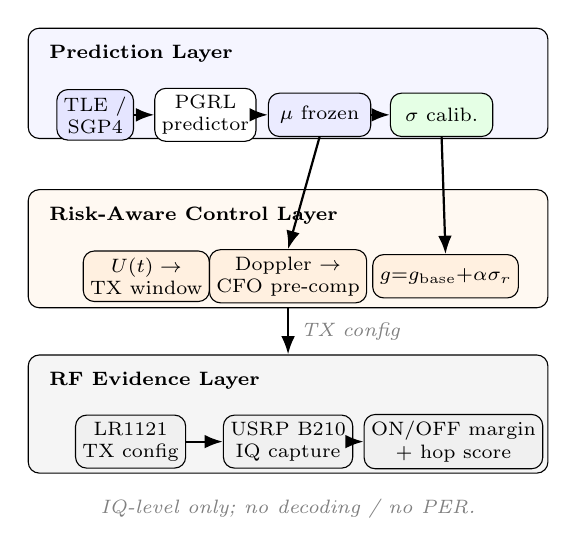
\begin{tikzpicture}[
      font=\footnotesize, >=Latex,
      band/.style={draw, rounded corners, inner sep=0pt},
      blk/.style={draw, rounded corners, align=center, font=\scriptsize, inner sep=2.5pt, minimum height=5.5mm, fill=white},
      ttl/.style={font=\scriptsize\bfseries, anchor=north west},
      ar/.style={->, thick},
      note/.style={font=\scriptsize\itshape, gray}
    ]
    % ===== Prediction Layer (top) =====
    \node[band, fill=blue!4, minimum width=66mm, minimum height=14mm] (P) at (3.3,5.0) {};
    \node[ttl] at ([xshift=1.5mm,yshift=-1mm]P.north west) {Prediction Layer};
    \node[blk, fill=blue!10] (tle)  at (0.85,4.6) {TLE /\\SGP4};
    \node[blk] (pred) at (2.25,4.6) {PGRL\\predictor};
    \node[blk, fill=blue!8,  minimum width=13mm] (mu) at (3.7,4.6) {$\mu$ frozen};
    \node[blk, fill=green!10,minimum width=13mm] (sg) at (5.25,4.6) {$\sigma$ calib.};
    \draw[ar] (tle) -- (pred);
    \draw[ar] (pred) -- (mu);
    \draw[ar] (mu) -- (sg);

    % ===== Risk-Aware Control Layer (middle) =====
    \node[band, fill=orange!5, minimum width=66mm, minimum height=15mm] (C) at (3.3,2.9) {};
    \node[ttl] at ([xshift=1.5mm,yshift=-1mm]C.north west) {Risk-Aware Control Layer};
    \node[blk, fill=orange!12] (uw)  at (1.5,2.55) {$U(t)\to$\\TX window};
    \node[blk, fill=orange!12] (cfo) at (3.3,2.55) {Doppler $\to$\\CFO pre-comp};
    \node[blk, fill=orange!12] (g)   at (5.3,2.55) {$g{=}g_{\text{base}}{+}\alpha\sigma_r$};

    % ===== RF Evidence Layer (bottom) =====
    \node[band, fill=gray!8, minimum width=66mm, minimum height=15mm] (R) at (3.3,0.8) {};
    \node[ttl] at ([xshift=1.5mm,yshift=-1mm]R.north west) {RF Evidence Layer};
    \node[blk, fill=gray!12] (cfg)  at (1.3,0.45) {LR1121\\TX config};
    \node[blk, fill=gray!12] (usrp) at (3.3,0.45) {USRP B210\\IQ capture};
    \node[blk, fill=gray!12] (evd)  at (5.4,0.45) {ON/OFF margin\\+ hop score};
    \draw[ar] (cfg) -- (usrp);
    \draw[ar] (usrp) -- (evd);

    % ===== inter-layer flow =====
    \draw[ar] (sg.south) -- (g.north);            % uncertainty -> guard
    \draw[ar] (mu.south) -- (cfo.north);          % mean -> Doppler/CFO + timing
    \draw[ar] (C.south) -- node[note,right=1pt]{TX config} (R.north);

    % note
    \node[note, anchor=north] at (3.3,-0.15) {IQ-level only; no decoding / no PER.};
    \end{tikzpicture}}
    \caption{Three-block cross-layer architecture. The \emph{Prediction Layer} maps TLE/SGP4 through a PGRL residual predictor to a frozen mean $\mu$ and a calibrated uncertainty $\sigma$. The \emph{Risk-Aware Control Layer} converts the radial uncertainty $\sigma_r$ into a guard $g=g_{\text{base}}+\alpha\sigma_r$, Doppler/CFO pre-compensation, and a transmit window via a utility $U(t)$, producing the LR1121 TX configuration. The \emph{RF Evidence Layer} captures the conducted LR1121-to-USRP B210 signal, reporting the TX-ON/OFF margin and hop-structure score (Fig.~\ref{fig:sdr}).}
    \label{fig:architecture}
\end{figure}

% ── Related Work ──────────────────────────────────────────────────────────────
\section{Related Work}
\label{sec:related}

\subsection{LR-FHSS for Direct-to-Satellite IoT}
LR-FHSS extends LoRaWAN for direct-to-satellite IoT by distributing transmit energy across a grid of narrow hopping bins, providing frequency diversity against the strong Doppler of LEO passes~\cite{semtech2023lrfhss,boquet2021lrfhss,hurn2023lrfhss}. Prior LR-FHSS satellite-IoT studies focus largely on the \emph{receiver side}---synchronization, detection, packet delivery, and reliability recovery once a transmission is present; real-world LR-FHSS packet-trace studies further show that fragment recovery and demodulation are a dedicated software-receiver problem~\cite{bukhari2023lrfhss}. In contrast, this work targets \emph{terminal-side} control: how orbital-prediction uncertainty should shape uplink guard and timing decisions before transmission.

\subsection{ML for LEO Orbit Prediction}
Analytical TLE propagators such as SGP4/SDP4~\cite{hoots1980models,vallado2007fundamentals} are deterministic and lightweight but accumulate timing and Doppler error with prediction horizon and TLE age. Machine-learning orbit work increasingly treats such a propagator as a physics anchor and learns residual corrections---via physics-informed networks for satellite state estimation~\cite{varey2024pinn} and learned LEO orbit prediction with exogenous variables~\cite{caldas2024leo}---but the common objective is trajectory accuracy as an end in itself. This work instead uses SGP4-anchored residual learning to expose a \emph{calibrated uncertainty} that drives communication-side control, rather than to minimize point error.

\subsection{LEO D2S Doppler and Uplink Control}
LEO non-terrestrial networking studies characterize the strong, time-varying Doppler of LEO passes and motivate pre-compensation and timing control at the terminal~\cite{3gpp2019tr38821,hurn2023lrfhss}, and uplink transmission-policy work for LoRa-based D2S IoT optimizes when and how a terminal transmits~\cite{alvarez2022uplink}. These works largely assume a fixed prediction or worst-case margin; we instead let a \emph{calibrated} per-pass uncertainty drive the margin. Uncertainty-aware control more broadly sizes safety margins to predicted risk rather than to a fixed bound; we apply this principle to LR-FHSS guard and timing using the calibrated PGRL uncertainty.

\subsection{Gap and Positioning}
Table~\ref{tab:related} summarizes the positioning. Unlike receiver-side LR-FHSS studies, we do not target detection, packet delivery, or gateway scalability; unlike ML orbit-prediction work, we do not treat trajectory accuracy as the primary metric; and unlike fixed-margin uplink-policy work, we adapt the margin to calibrated per-pass uncertainty. Our contribution is the \emph{cross-layer connection}: converting SGP4-anchored, calibrated uncertainty into terminal-side risk-aware LR-FHSS guard control.

\begin{table}[htbp]
\small
\caption{Positioning Relative to Prior Art}
\label{tab:related}
\begin{tabular}{p{2.0cm}p{2.6cm}p{2.7cm}}
\toprule
Category & Typical focus & This work's difference \\
\midrule
LR-FHSS DtS analysis & Packet delivery / outage & No prediction-driven uplink control \\
LR-FHSS transceiver & Receiver sync / detection & Terminal-side pre-transmission control \\
ML orbit prediction & Trajectory accuracy & Calibrated uncertainty for control \\
\midrule
\textbf{This work} & Calibrated uncertainty $\rightarrow$ risk-aware guard & Cross-layer terminal design \\
\bottomrule
\end{tabular}
\end{table}

% ── Background and System Model ───────────────────────────────────────────────
\section{Background and System Model}
\label{sec:system}

\subsection{LEO D2S Channel Characteristics}
During a typical LEO pass at $\sim$600~km altitude, the one-way Doppler reaches tens of kHz (order $20$~kHz at 868~MHz, $\sim$50~kHz at S-band) with the largest Doppler rate near closest approach; exact values scale with carrier frequency and pass geometry. The Doppler shift is modeled as
\begin{equation}
f_D(t) = -\frac{v_r(t)}{c}\,f_c
\label{eq:doppler}
\end{equation}
where $v_r(t)$ is the radial velocity (positive when satellite recedes) and $c$ is the speed of light. The residual CFO after pre-compensation is
\begin{equation}
f_{\mathrm{res}}(t) = f_D(t) - \hat{f}_D(t) + f_{\mathrm{osc}},
\label{eq:residual_cfo}
\end{equation}
where $\hat{f}_D$ is the predicted Doppler and $f_{\mathrm{osc}}$ is the terminal oscillator offset. In our LR-FHSS-inspired proxy, the available bandwidth is discretized into $N_f$ hopping bins. The bin width is treated as an evaluation parameter rather than a complete standard-compliant receiver model. In this simplified reception proxy, reliable hop reception is modeled as $|f_{\mathrm{res}}|$ after pre-compensation remaining small relative to the bin width; this is a proxy criterion, not a standard-compliant receiver model.

\subsection{SGP4/SDP4 Orbital Propagation}
SGP4/SDP4~\cite{hoots1980models} propagates Two-Line Element (TLE) sets to produce Cartesian position and velocity at any epoch. The algorithm is deterministic and computationally lightweight but accumulates RMS timing errors of 1--4~s and Doppler errors of $>5$~kHz over prediction horizons of 30--120~min, depending on TLE age. These errors are non-Gaussian and time-correlated, which limits the effectiveness of naive uncertainty estimation on top of SGP4 output.

\subsection{PGRL Architecture}
PGRL augments SGP4 with a SIREN (sinusoidal representation network) residual predictor. The input is the query time-since-epoch together with the SGP4-derived normalized orbital state/elements; the network emits a stacked $12$-vector $[\boldsymbol{\mu}\,(6),\ \log\boldsymbol{\sigma}^2\,(6)]$. The mean head $\boldsymbol{\mu}$ gives the corrected position/velocity state (normalized by distance/velocity units $\mathrm{DU}{=}10^4$~m, $\mathrm{VU}{=}10$~m/s), and the parallel log-variance head $\log\sigma_i^2$ gives a per-axis uncertainty. This is a heteroscedastic-uncertainty head, not a Bayesian posterior: there is no weight sampling, ensemble, or variational inference. The \emph{deterministic} predictor is trained earlier with a state MSE plus a physics-inspired regularizer penalizing departures from Keplerian energy $E=-\mu/(2a)$ and angular-momentum $|\mathbf{h}|=\sqrt{\mu a(1-e^2)}$ conservation.

\emph{Uncertainty-head fine-tuning (Stage 3E).} Starting from the trained deterministic checkpoint, the mean head is \emph{frozen} and the objective $\mathcal{L}=\mathcal{L}_{\text{MSE}}+\mathcal{L}_{\text{phys}}+0.05\,\mathcal{L}_{\text{NLL}}$ is minimized. The MSE and physics terms are retained for continuity with the deterministic stage but, with the mean frozen, update no trainable parameter, so only the log-variance layer is updated, through the Gaussian NLL term
\begin{equation}
\mathcal{L}_{\text{NLL}} = \frac{1}{N}\sum_{n=1}^{N}\sum_{i=1}^{3}\left[
  \log\sigma_{n,i}^2 + \frac{(y_{n,i} - \mu_{n,i})^2}{\sigma_{n,i}^2}
\right],
\label{eq:nll}
\end{equation}
where $\mu_{n,i},\sigma_{n,i}$ are the (frozen) mean and learned per-axis standard deviation. The log-variance layer is initialized to $\log((10/\mathrm{DU})^2)$ (an initial per-axis $\sigma\approx 10$~m in reported metres, $\mathrm{DU}$ the distance unit) and converges to a mean axis $\sigma\approx 3.01$~m. Because the mean head is frozen, the point prediction---and therefore the deterministic accuracy---is unchanged by this stage. The learned uncertainty is thus a calibrated \emph{position-domain} ($\sigma$ in metres) estimate, not a directly trained timing (ms) or Doppler (Hz) uncertainty.

\emph{Coverage metric.} Calibration is assessed by Mahalanobis chi-square coverage: for each sample $z^2=\sum_i (e_i/\sigma_i)^2$ with per-axis error $e_i$. Under a calibrated $3$-DoF Gaussian, the 68\% and 95\% credible regions correspond to thresholds $z^2\le 3.506$ and $z^2\le 7.815$; the empirical coverage is the fraction of samples below each threshold (Sec.~\ref{sec:eval}).

% ── PGRL Orbital Predictor ────────────────────────────────────────────────────
\section{PGRL Orbital Predictor}
\label{sec:pgrl}

The PGRL predictor receives a TLE epoch and exposes a structured output with:
\begin{itemize}
  \item pass-start timing error (relative to SGP4-estimated AOS);
  \item residual Doppler and Doppler-rate error (after SGP4 compensation);
  \item one-sigma timing and Doppler uncertainty;
  \item a link-opportunity score (Doppler, timing, and energy cost); and
  \item a recommended guard time (minimum guard interval at $3.5\sigma$).
\end{itemize}

The trained uncertainty head emits a per-axis \emph{position-domain} standard deviation (in metres); the timing- and Doppler-domain $\sigma$ fields above are schema conveniences derived under the simulation mapping of Sec.~\ref{sec:uplink} and are not directly trained quantities. The uncertainty head maintains a near-calibrated scale without post-hoc rescaling (Sec.~\ref{sec:eval}); online/continual refinement is out of scope for this paper.

% ── Uplink Control ────────────────────────────────────────────────────────────
\section{LR-FHSS Uplink Control}
\label{sec:uplink}

\subsection{Risk-Aware Guard-Band Policy}
\label{sec:guard}
The calibrated position-domain uncertainty is used to size the guard margin to the actual prediction risk. Let $\sigma_r$ be the calibrated radial standard deviation (in metres) from the uncertainty head. The risk-aware guard is
\begin{equation}
g_{\text{uncertain}} = g_{\text{base}} + \alpha\,\sigma_r,
\label{eq:riskguard}
\end{equation}
where $\alpha\ge 0$ scales the uncertainty contribution. The base guard $g_{\text{base}}$ is the $95$th-percentile position residual (a deterministic worst-case margin), and $\sigma_r=\lVert(\sigma_x,\sigma_y,\sigma_z)\rVert$ is the calibrated radial position uncertainty from the log-variance head. With $\alpha=0$ the policy reduces to the fixed deterministic baseline; increasing $\alpha$ widens the guard in proportion to the predicted per-sample uncertainty. Each $\alpha$ is scored by an \emph{outage proxy} $\rho=\Pr[e_r>g_{\text{uncertain}}]$ (residual error exceeding the guard), a \emph{success proxy} $1-\rho$, a normalized guard overhead $\bar g=\mathbb{E}[g_{\text{uncertain}}]/\mathbb{E}[g_{\text{base}}]$, and a risk-adjusted reward
\begin{equation}
R = (1-\rho) - \lambda\,(\bar g - 1), \qquad \lambda = 0.1.
\label{eq:reward}
\end{equation}
We sweep $\alpha\in\{0.00,0.25,0.50,0.75,1.00\}$. These are control proxies, not measured packet-error rates.

\subsection{Doppler Pre-Compensation (Simulation/Proxy)}
As a separate control-framework component (a \emph{simulation/proxy assumption}, not part of the Stage~3E/3F/4 trained-model evidence), the \texttt{compensated\_tx\_frequency} function adjusts the nominal carrier $f_c$ using a predicted Doppler shift $\hat{f}_d$ and rate $\hat{f}_d'$:
\begin{equation}
f_{\text{TX}} = f_c - \hat{f}_d - \frac{\hat{f}_d'}{2}\,T_{\text{burst}},
\end{equation}
with $T_{\text{burst}}$ the burst duration. Under the simulation assumptions of Sec.~\ref{sec:eval}, tighter residual CFO keeps hop energy within an LR-FHSS bin; we report only proxy RF-quality indicators (EVM proxy, grid orthogonality) and do not measure PER.

\subsection{TX Timing Selection}
The \texttt{select\_tx\_time} function scores candidate transmission windows using a weighted utility:
\begin{equation}
U(t) = \alpha \cdot \text{link\_score}(t) - \beta \cdot |f_d'(t)| - \gamma \cdot E_{\text{idle}}(t)
\end{equation}
where the utility weights are tunable (the guard scale $\alpha$ of Eq.~\ref{eq:riskguard} is distinct from these weights). The optimizer selects the window with maximum $U(t)$ within a 6-hour planning horizon, balancing link quality, Doppler rate, and energy expenditure. Algorithm~\ref{alg:control} summarizes the end-to-end terminal-side procedure.

\begin{figure}[t]
\centering
\setlength{\fboxsep}{5pt}
\fbox{\begin{minipage}{0.92\columnwidth}
\footnotesize
\textbf{Algorithm 1:} Uncertainty-Aware LR-FHSS Uplink Control\\[2pt]
\textbf{Input:} TLE, query window $\mathcal{T}$, trained PGRL, base guard $g_{\text{base}}$, scale $\alpha$\\
\textbf{Output:} LR-FHSS TX configuration
\begin{enumerate}\setlength\itemsep{1pt}\setlength\parskip{0pt}
  \item Propagate the SGP4 state over $\mathcal{T}$.
  \item Predict residual correction $\mu$ and uncertainty $\sigma$ with PGRL.
  \item Compute radial uncertainty $\sigma_r=\lVert(\sigma_x,\sigma_y,\sigma_z)\rVert$.
  \item Set guard $g=g_{\text{base}}+\alpha\,\sigma_r$.
  \item Estimate Doppler $\hat f_d$ and residual CFO $f_{\text{res}}$.
  \item Score candidate TX windows by utility $U(t)$.
  \item Select $t^\star=\arg\max_t U(t)$ and configure the LR1121 (center frequency, hop grid, guard $g$, CFO pre-compensation).
\end{enumerate}
\end{minipage}}
\caption{Terminal-side uncertainty-aware uplink control procedure.}
\label{alg:control}
\end{figure}

% ── Evaluation ────────────────────────────────────────────────────────────────
\section{Evaluation}
\label{sec:eval}

\subsection{Experimental Setup}
The Stage~3E/3F/4 results are produced by the offline evaluation scripts under \url{scripts/} (uncertainty-head fine-tuning, temperature calibration, and risk-aware control ablation) applied to the deterministic checkpoint, with seed~$=42$; trained checkpoints reside on the training machine and are not included in the repository. Reported metres use $e_m = e_{\text{norm}}\cdot\mathrm{DU}$. The risk-aware ablation (Eq.~\ref{eq:riskguard}) defines the outage proxy as the fraction of samples with $e_r>g_{\text{uncertain}}$, the success proxy as its complement, and the reward as $\text{success}-\lambda(\,\overline{g}-1)$ with energy weight $\lambda=0.1$ and $\overline{g}$ the guard normalized to the $\alpha{=}0$ baseline. As \emph{separate control-framework simulation proxies} (Monte Carlo, seed~42; not Stage~3E/3F/4 trained-model evidence) we additionally report an LR-FHSS 64-bin grid-orthogonality proxy and a QPSK EVM proxy at SNR$=40$~dB; these are RF-quality indicators only and are not LR-FHSS PER.

\subsection{Calibrated Uncertainty and Risk-Aware Control}

\begin{figure}[t]
    \centering
    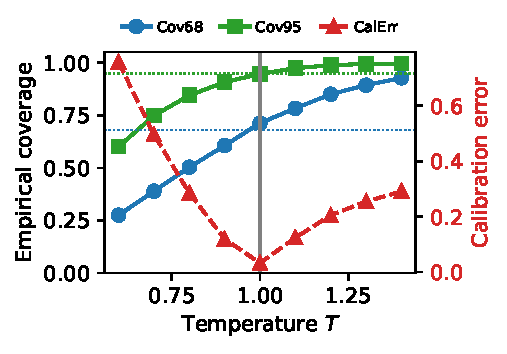
\includegraphics[width=0.82\linewidth]{figures/fig2_temperature_calibration.pdf}
    \caption{Stage~3F post-hoc temperature calibration. Empirical Cov68/Cov95 and calibration error vs.\ scalar temperature $T$; RMSE is invariant at 5.35~m (frozen mean). Best calibration at $T=1.0$ (Cov68/Cov95 $=0.713/0.947$, CalErr $=0.0331$), i.e.\ no post-hoc rescaling needed.}
    \label{fig:tempcal}
\end{figure}

\begin{figure}[t]
    \centering
    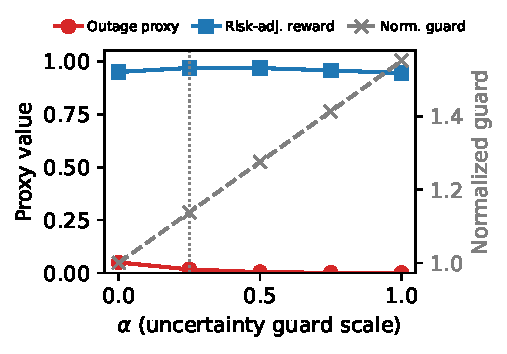
\includegraphics[width=0.82\linewidth]{figures/fig3_risk_aware_ablation.pdf}
    \caption{Stage~4 risk-aware guard ablation over $\alpha$ (Eq.~\ref{eq:riskguard}). Outage/success/reward are control proxies (not PER); RMSE is fixed at 5.35~m and collision proxy is $0.000$ for all $\alpha$. Risk-adjusted reward peaks at $\alpha=0.25$.}
    \label{fig:risk}
\end{figure}

\begin{figure}[t]
    \centering
    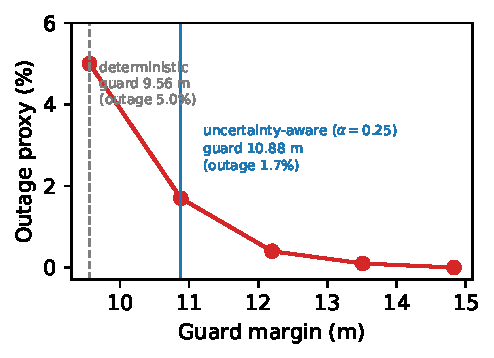
\includegraphics[width=0.82\linewidth]{figures/fig4_guard_residual_distribution.pdf}
    \caption{Outage proxy vs.\ guard margin from the Stage~4 $\alpha$ sweep (operating points; per-sample residuals are not exported). Deterministic guard (9.56~m, $\alpha{=}0$) gives 5.0\% outage; the uncertainty-aware guard (10.88~m, $\alpha{=}0.25$) gives 1.7\%.}
    \label{fig:guardres}
\end{figure}

\emph{Stage 3E (uncertainty-head fine-tuning).} With the mean head frozen, deterministic accuracy is unchanged: position RMSE remains 5.35~m and the fraction of predictions within 5~m remains 61.3\%. The log-variance head learns a metre-scale uncertainty, with the mean per-axis $\sigma$ moving from an initialized $\approx 10$~m to $\approx 3.01$~m, yielding non-trivial Mahalanobis coverage.

\emph{Stage 3F (temperature calibration).} Fig.~\ref{fig:tempcal} sweeps a scalar temperature $T$ applied as $\log\sigma^2_T=\log\sigma^2+2\log T$, which is equivalent to scaling the predicted standard deviation by $T$ ($\sigma_T=T\sigma$). RMSE is invariant to $T$ (the mean is frozen). The best calibration error occurs at $T=1.0$ (Cov68/Cov95 $=0.713/0.947$, CalErr $=0.0331$), confirming that the learned uncertainty scale is already near-optimal \emph{without} post-hoc rescaling.

\emph{Sensitivity to the uncertainty scale.} Table~\ref{tab:sens} reports the coverage and calibration error as the uncertainty scale $T$ (equivalently the $\sigma$ multiplier) is varied around the operating point. Under-scaling ($T<1$) sharply under-covers (e.g.\ $T=0.6$ gives Cov68 $=0.275$), while over-scaling ($T>1$) over-covers; both raise the calibration error monotonically away from $T=1.0$. The control behavior follows directly through Eq.~\ref{eq:riskguard}, since $\sigma_r$ scales with $T$: too small a scale under-sizes the guard (higher outage), too large a scale inflates the guard overhead. The near-unity optimum indicates the learned head needs no manual scale tuning.

\begin{table}[t]
\centering
\small
\caption{Sensitivity to the uncertainty scale $T$ ($\sigma_T=T\sigma$); RMSE $=5.35$~m for all $T$ (frozen mean). Values from the Stage~3F sweep.}
\label{tab:sens}
\begin{tabular}{cccc}
\toprule
scale $T$ & Cov68 & Cov95 & CalErr \\
\midrule
0.6 & 0.275 & 0.601 & 0.7569 \\
0.8 & 0.503 & 0.845 & 0.2852 \\
\textbf{1.0} & \textbf{0.713} & \textbf{0.947} & \textbf{0.0331} \\
1.2 & 0.850 & 0.988 & 0.2053 \\
1.4 & 0.928 & 0.996 & 0.2909 \\
\bottomrule
\end{tabular}
\end{table}

\emph{Stage 4 (risk-aware guard ablation).} Fig.~\ref{fig:risk} sweeps $\alpha$ in Eq.~\ref{eq:riskguard}, and Fig.~\ref{fig:guardres} shows the resulting outage-vs-guard operating points. RMSE is fixed at 5.35~m across all $\alpha$, confirming the point predictor is untouched. Relative to the deterministic baseline ($\alpha{=}0$: outage 5.0\%, reward 0.9500), the uncertainty-aware policy at $\alpha{=}0.25$ reduces the outage proxy to 1.7\% (a $3\times$ reduction) and raises the success proxy to 0.9828 and the reward to 0.9690, at a guard overhead of $+13.8\%$. Larger $\alpha$ drives outage lower still (Table~\ref{tab:alpha}) but the risk-adjusted reward peaks at $\alpha{=}0.25$, since the guard-overhead penalty eventually outweighs the diminishing outage gain. The collision proxy is $0.000$ for all $\alpha$, so outage---not collision---is the binding robustness metric in this proxy setup; we therefore do not claim collision reduction.

\begin{table}[t]
\centering
\small
\caption{Stage~4 risk-aware guard ablation (control proxies, not PER). RMSE $=5.35$~m and collision proxy $=0.000$ for all $\alpha$.}
\label{tab:alpha}
\begin{tabular}{cccccc}
\toprule
$\alpha$ & guard (m) & $\bar g$ & outage & success & reward $R$ \\
\midrule
0.00 & 9.56  & 1.000 & 0.050 & 0.9500 & 0.9500 \\
\textbf{0.25} & \textbf{10.88} & \textbf{1.138} & \textbf{0.017} & \textbf{0.9828} & \textbf{0.9690} \\
0.50 & 12.20 & 1.276 & 0.004 & 0.9961 & 0.9685 \\
0.75 & 13.51 & 1.414 & 0.001 & 0.9989 & 0.9575 \\
1.00 & 14.83 & 1.552 & 0.000 & 1.0000 & 0.9448 \\
\bottomrule
\end{tabular}
\end{table} The separate simulation proxies give a QPSK EVM proxy of $\approx 67\%$ and a grid orthogonality of $0.706$ at 300~Hz residual CFO, indicating that deployment-grade receiver validation would require residual-CFO tracking and a decoded receiver.

\subsection{Validation Scope}
This work evaluates terminal-side prediction and control. The outage, success, reward, EVM, and grid-orthogonality figures are simulation/proxy indicators rather than measured PER, and the heteroscedastic head is a calibrated log-variance output, not a Bayesian posterior. The conducted LR1121/USRP capture validates IQ-level signal presence and hop-like spectral structure; no gateway-class decoder is implemented. Position-domain uncertainty is mapped to timing/frequency control margins through the proxy model of Sec.~\ref{sec:uplink}, leaving a modeling gap between the two domains. Online adaptation, decoded packet delivery, and PER measurement are future work.

% ── Conducted IQ-Level RF Evidence ───────────────────────────────────────────
\section{Conducted IQ-Level RF Evidence}
\label{sec:hardware}

This section supports the transmitter-configuration and signal-observability path of Fig.~\ref{fig:architecture}; it characterizes RF signal presence, not receiver performance.

\subsection{Semtech LR1121 TX Path}
A Semtech LR1121/LR11xx dev-kit running SWDM001 firmware~\cite{swdm001} transmits LR-FHSS bursts at 868~MHz, 10~dBm. A configuration script converts the PGRL-driven control output into the TX configuration (center frequency, TX power, hopping-grid parameters, guard time, Doppler pre-compensation flags), and the device UART log confirms bursts were emitted.

\subsection{Conducted USRP IQ Capture}
A USRP B210 (1~MHz sample rate, 45~dB gain, $\sim$10~s) connected by coax to the LR1121 captures raw IQ under a TX-ON/TX-OFF differential protocol. Fig.~\ref{fig:sdr} shows the max-hold spectra: the TX-ON capture exceeds the TX-OFF reference by 9.82~dB with discrete hop tones, passing the shared signal-detection test (LR-FHSS-candidate score 0.76, status \emph{signal-detected}; DC/LO guard band excluded). This confirms IQ-level RF signal presence consistent with an LR-FHSS-configured transmission under conducted capture; the raw IQ is held locally and is not committed.

\begin{figure}[t]
    \centering
    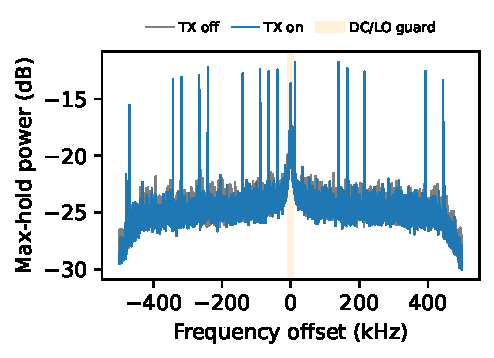
\includegraphics[width=0.82\linewidth]{figures/fig5_sdr_capture_validation.pdf}
    \caption{Conducted LR1121$\rightarrow$USRP B210 IQ capture at 868~MHz: TX-ON vs TX-OFF max-hold spectrum from the raw IQ ($\Delta=9.82$~dB; DC/LO guard shaded). IQ-level RF signal detection only --- not decoding, packet delivery, or PER.}
    \label{fig:sdr}
\end{figure}

\subsection{Offline IQ-Structure Analysis}
As additional \emph{structural} evidence, an offline IQ-structure analysis script (\url{scripts/analyze_lrfhss_iq_structure.py}; summary under \url{docs/lrfhss_iq_structure_stage5/}) detects sparse, multi-frequency candidate bursts on the same capture: 101 candidate bursts across 19 occupied frequency bins at $\approx$12\% time occupancy, with a bounded heuristic structure score of $\approx$0.845, consistent with LR-FHSS-like frequency hopping. This is a structural heuristic, not a decoder; receiver-side decoding remains a dedicated gateway-class or software-receiver problem~\cite{bukhari2023lrfhss}.

% ── Conclusion ────────────────────────────────────────────────────────────────
\section{Conclusion}
\label{sec:conclusion}

We presented a calibrated uncertainty-driven cross-layer framework that turns SGP4-anchored PGRL prediction uncertainty into terminal-side LR-FHSS guard, timing, and Doppler control. With the deterministic mean frozen, the calibrated uncertainty head preserves the 5.35~m position RMSE and is near-calibrated without rescaling ($T{=}1.0$, Cov68/Cov95 $=0.713/0.947$), and the risk-aware guard policy lowers the outage proxy from 5.0\% to 1.7\% at 13.8\% guard overhead. A conducted LR1121-to-USRP B210 capture confirms IQ-level RF signal presence with a 9.82~dB margin. Future work will close the receiver-in-the-loop gap using gateway-class LR-FHSS decoding and measured PER.

% ── References ───────────────────────────────────────────────────────────────
\bibliographystyle{IEEEtran}
\bibliography{refs}

\end{document}